\documentclass{beamer}


\usepackage[french,english]{babel}

\usepackage[T1]{fontenc}

\usepackage[utf8]{inputenc}


\usetheme{Warsaw}
\title{Apprentissage et résultats}

\author{Clément Legrand}
\date{21 Juin 2018}

\begin{document}


\begin{frame}[plain]
\titlepage
\end{frame}

\section{Apprentissage}

\subsection{Description}

\begin{frame}{Description}
\begin{block}{Base de départ}
Les solutions données par CW.
\begin{itemize}
\item Tirage au sort de N triplets ($\lambda$, $\mu$, $\nu$);
\item Calcul de toutes les valeurs possibles.
\end{itemize}
\end{block}

\begin{block}{Base d'apprentissage}
On ne garde qu'une partie de la base générée pour apprendre.
\begin{itemize}
\item On garde $10\%$ des meilleurs solutions (quantité privilégiée);
\item On garde les solutions qui ont un coût inférieur à $c_{min} + \frac{c_{max}-c_{min}}{10}$ (qualité privilégiée).
\end{itemize}
\end{block}
\end{frame}

\begin{frame}{Protocole}

\begin{exampleblock}{Protocole}
\begin{itemize}
\item Génération de la base de départ
\item Génération de la base d'apprentissage
\item On initialise une matrice MAT de taille $n^2$
\item Pour chaque arête (a,b) on incrémente la valeur MAT[a][b] (si a>b, on commence par échanger a et b)
\item On regarde si les arêtes obtenues sont effectivement dans la solution optimale.
\end{itemize}
\end{exampleblock}

\begin{block}{Choix des arêtes}
\begin{itemize}
\item On conserve (a,b) si MAT[a][b] dépasse une certaine valeur (Requis);
\item On conserve les k premières arêtes en triant selon les valeurs de MAT (Rang).
\end{itemize}
\end{block}

\end{frame}

\subsection{Résultats apprentissage}

\begin{frame}{Instance test}
Tous les tests qui suivent n'ont été réalisés que sur l'instance A-n37-k06.

La solution employée pour comparer les résultats est celle de la littérature.

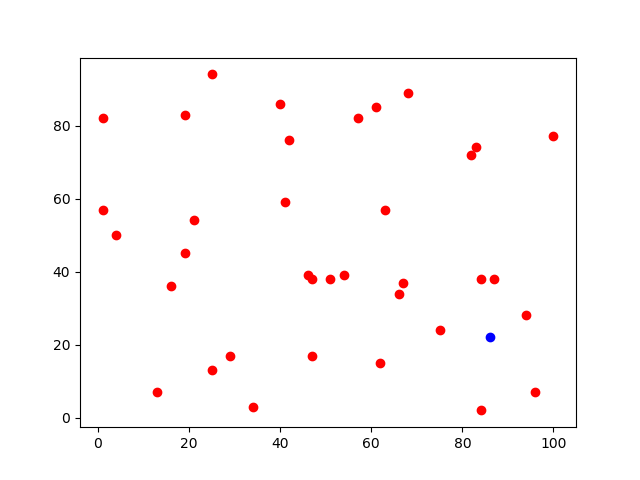
\includegraphics[scale=0.3]{instance3706.png}
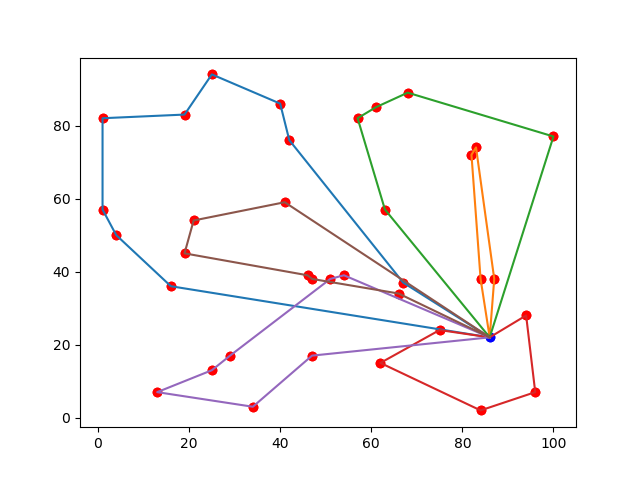
\includegraphics[scale=0.3]{best3706.png}

Pour chaque test on effectue 5 itérations.
\end{frame}

\begin{frame}{Résultats avec critère Requis}
\emph{L$_{lb}$} est la taille de la base d'apprentissage. 

\centering
\begin{tabular}{|c|c|c|c|c|c|}
   \hline
   Taille base & Requis & Quan$_{10}$ & Qual$_{10}$ & Tout & Time (s)\\
   \hline
   100 & L$_{lb}$/2 & 0.71 & 0.73 & 0.72 & 2.54 \\
   \hline
   500 & L$_{lb}$/2 & 0.75 & 0.73 & 0.71 & 12.7 \\
   \hline
   1000 & L$_{lb}$/2 & 0.73 & 0.75 & 0.71 & 25.6 \\
   \hline
   \hline
   100 & 3L$_{lb}$/4 & 0.90 & 0.85 & 1.0 & 2.57 \\
   \hline
   500 & 3L$_{lb}$/4 & 0.88 & 0.81 & 1.0 & 12.8 \\
   \hline
   1000 & 3L$_{lb}$/4 & 0.92 & 0.83 & 1.0 & 25.4 \\
   \hline
\end{tabular}

\begin{itemize}
\item Quan$_{10}$ et Qual$_{10}$ renvoient en moyenne 22 arêtes lorsque Requis vaut L$_{lb}$/2, et 15 arêtes lorsque Requis vaut 3L$_{lb}$/4;
\item Tout renvoie en moyenne respectivement 15 arêtes et 6 arêtes.
\end{itemize}
\begin{exampleblock}{Remarque}
Quan$_{10}$ semble être la base la plus adaptée pour le critère de choix Requis.
\end{exampleblock}
\end{frame}

\begin{frame}{Résultats avec critère Rang}

\centering
\begin{tabular}{|c|c|c|c|c|c|}
   \hline
   Taille base & Rang max & Quan$_{10}$ & Qual$_{10}$ & Tout & Time (s)\\
   \hline
   100 & 10 & 0.90 & 0.90 & 0.96 & 2.52 \\
   \hline
   500 & 10 & 0.90 & 0.98 & 0.92 & 12.5 \\
   \hline
   1000 & 10 & 0.92 & 0.98 & 0.98 & 25.4 \\
   \hline
   \hline
   100 & 20 & 0.79 & 0.79 & 0.73 & 2.57 \\
   \hline
   500 & 20 & 0.82 & 0.81 & 0.76 & 12.9 \\
   \hline
   1000 & 20 & 0.84 & 0.81 & 0.75 & 25.5 \\
   \hline
\end{tabular}

\begin{exampleblock}{Remarque}
Qual$_{10}$ semble être la base la plus adaptée pour le critère de choix Rang.
\end{exampleblock}

\end{frame}


\begin{frame}{Résultats avec toutes les SI}
Temps de calcul pour avoir la base : 37.5 s

\centering
\begin{tabular}{|c|c|c|c|}
   \hline
   Requis & Quan$_{10}$ & Qual$_{10}$ & Time (s)\\
   \hline
   L$_{lb}$/2 & 0.73 & 0.77 & 0.076 \\
   \hline
   3L$_{lb}$/4 & 0.93 & 0.89  & 0.077 \\
   \hline
\end{tabular}

Quan$_{10}$ reste la base la plus performante pour le critère Requis.

\begin{tabular}{|c|c|c|c|}
   \hline
   Rang max & Quan$_{10}$ & Qual$_{10}$ & Time (s)\\
   \hline
   10 & 0.9 & 1.0 & 0.074 \\
   \hline
   20 & 0.85 & 0.85 & 0.076 \\
   \hline
\end{tabular}

Qual$_{10}$ reste la base la plus performante pour le critère Rang.
\end{frame}

\section{Intégration de la connaissance dans un algorithme}

\subsection{Présentation algorithme}
\begin{frame}{Algorithme actuel}

\begin{center}
\begin{tabular}{|c|}
	\hline
 	\textbf{Apprentissage} \\
   \hline
   \textbf{Boucle sur $(\lambda, \nu, \mu)$} \\
   \hline
   \hline
   Initialisation$_{CW}$ + \textbf{utilisation apprentissage} \\
   \hline
   LK$_{BI-O}$ \\
   \hline
   \hline
   Condition d'arrêt : 1500 itérations depuis la dernière amélioration  \\
   \hline
   Compute worst edge \\
   \hline
   EC$_{BI-O}$ \\
   \hline
   LK$_{BI-O}$ \\
   \hline
   CE$_{FI-O}$ \\
   \hline
   LK$_{BI-O}$ \\
   \hline
   Itérations spéciales \\
   \hline
   \hline

\end{tabular}
\end{center}
\end{frame}

\subsection{Résultats}

\begin{frame}{Premiers résultats}

\flushleft
\begin{tabular}{|c|c|c|c|c|}
   \hline
   Méthode & A-n32-k05 & A-n34-k05 & A-n37-k06 & Time (s)\\
   \hline
   Sans & 791.57 & 1 & 1& 1  \\
   \hline
   Quan$_{10}$ & 791.57 & 795.88 & 950.8 & 1   \\
   \hline
   Qual$_{10}$ & 791.57 & 788.98 & 950.8 & 1  \\
   \hline
\end{tabular}


\end{frame}

\end{document}